% IEEE TGRS manuscript: IDR reproduction and seismic adaptation.
% Build (from report/):  pdflatex main; bibtex main; pdflatex main; pdflatex main
% Figures: python scripts/make_figures.py ; tables: python scripts/make_tables.py (run from repro/)
\documentclass[journal]{IEEEtran}
\usepackage[T1]{fontenc}
\usepackage{amsmath,amssymb}
\usepackage{graphicx}
\usepackage{booktabs,multirow}
\usepackage{algorithm}
\usepackage{algpseudocode}
\usepackage{cite}
\usepackage{microtype}
\usepackage{xcolor}
\usepackage[hidelinks]{hyperref}
\graphicspath{{figures/}}
\newcommand{\ie}{i.e.,\ }
\newcommand{\eg}{e.g.,\ }
\newcommand{\todo}[1]{\textcolor{red}{[TODO: #1]}}

\begin{document}
\title{Self-Supervised Seismic Random-Noise Attenuation by Iterative Data Refinement: Reproduction of Fast IDR and Application to Synthetic and Field Data}

\author{\todo{author names and affiliations}%
\thanks{Manuscript draft, 28 November 2026.}}

\markboth{IEEE Transactions on Geoscience and Remote Sensing (draft)}{}
\maketitle

\begin{abstract}
Iterative data refinement (IDR) trains a denoiser without clean targets: it builds noisier--noisy pairs from single noisy observations and a noise model, then repeatedly replaces the targets with the network's own estimates. We reproduce Fast IDR on images under the protocol stated in the paper. The method ranking is recovered and Gaussian-noise PSNR is within 0.30--0.54\,dB of the published values, but the reported parity with supervised training is not: Fast IDR trails it by 0.12--0.20\,dB in every setting and seed. We then transfer the method to seismic data with four noise analogues (white, band-limited, spikes, dead traces) and three SEG synthetic models. For additive noise, Fast IDR comes within 1.2\,dB of supervised training, beats bandpass filtering, $f$-$x$ deconvolution and oracle-$\sigma$ BM3D, and beats supervised training by 0.8--2.2\,dB on unseen processing versions of Marmousi2. On four public field datasets (2D/3D, land/marine), Fast IDR trained on the target survey is the best method in semi-synthetic tests (+1.1 to +2.7\,dB over the best classical method). On real noise, it removes noise with low leakage on the 2D land line, removes it only partially on the 2D marine line, and removes almost nothing from post-stack 3D volumes, whose residual noise is largely coherent.
\end{abstract}

\begin{IEEEkeywords}
Seismic denoising, self-supervised learning, iterative data refinement, noise modeling, reproducibility.
\end{IEEEkeywords}

%=====================================================================
\section{Introduction}
\IEEEPARstart{C}{lassical} seismic denoisers, such as $f$-$x$ deconvolution~\cite{canales1984fx}, bandpass and median filters, and BM3D~\cite{dabov2007bm3d,makinen2020bm3d}, need per-survey tuning and trade residual noise against signal leakage. Supervised CNNs~\cite{zhang2017dncnn,yu2019dnseis} need clean targets, which field data lack. Synthetic training data fill that gap only at the cost of a domain gap.

Self-supervised methods relax this requirement in different ways:
\begin{itemize}
\item Noise2Noise (N2N)~\cite{lehtinen2018n2n} needs two aligned noisy realizations of the same signal, which seismic surveys rarely provide.
\item Blind-spot methods (N2V~\cite{krull2019n2v}, N2S~\cite{batson2019n2s}, DBSN~\cite{wu2020dbsn}) assume noise that is independent between pixels, which band-limited or trace-coherent seismic noise violates.
\item Deep image prior (DIP)~\cite{ulyanov2018dip} fits one network per image and needs early stopping.
\item Noisier2Noise (Nr2N)~\cite{moran2020nr2n} and IDR~\cite{zhang2022idr} need only a noise model that can be sampled, which suits seismic data, whose noise families can be parameterized per survey.
\end{itemize}
Self-supervised seismic denoising has been studied~\cite{birnie2021ssl}, but, to our knowledge, IDR has not been reproduced or tested on field seismic data.

We contribute:
\begin{enumerate}
\item a protocol-faithful reproduction of Fast IDR with three seeds and an attribution of the gap to the published numbers;
\item seismic analogues of the paper's noise families, tested on three SEG synthetic models with classical baselines and a cross-processing test;
\item an application to four public field datasets;
\item released code, logs and weights, from which every table and figure is regenerated by script.
\end{enumerate}

%=====================================================================
\section{Methods of Analysis}\label{sec:methods}
\subsection{Data Bias and Iterative Data Refinement}
Following~\cite{zhang2022idr}, let $y_i$ be the clean signal, $n_i$ a noise sample, and $x_i=y_i+n_i$ the observation (``$+$'' denotes applying the noise model). Supervised training uses pairs $\{(y_i+n_i,y_i)\}$; without $y_i$ one can use noisier--noisy pairs $\{(x_i+n_i,x_i)\}$. Zhang et al.\ call the resulting train--inference mismatch \emph{data bias}. Their pilot study reports that (i)~noisier--noisy training generalizes to real noisy inputs, and (ii)~training sets closer to noisy--clean pairs give better denoisers. We did not repeat the pilot study. IDR reduces the bias by training $F_0$ on noisier--noisy pairs and then, for $m=1,\dots,M$,
\begin{equation}
F_{m} \leftarrow \bigl\{\,F_{m-1}(x_i)+n_i,\; F_{m-1}(x_i)\,\bigr\},
\label{eq:idr}
\end{equation}
so the targets $x_i^{(m)}=F_{m-1}(x_i)$ approach $y_i$ (Fig.~\ref{fig:framework}). Inference applies $F_M$ once; repeated application would over-smooth.

\begin{figure}[!t]
\centering
\IfFileExists{figures/idr_framework.pdf}{\includegraphics[width=\columnwidth]{idr_framework.pdf}}{%
\IfFileExists{figures/idr_framework.png}{\includegraphics[width=\columnwidth]{idr_framework.png}}{%
\fbox{\parbox[c][3.2cm][c]{0.94\columnwidth}{\centering\small Missing asset: \texttt{report/figures/idr\_framework.pdf}\\(Fig.~3 of arXiv:2111.14358, file \texttt{v3.png} in its source)}}}}
\caption{Overview of IDR. Reproduced from Zhang et al.~\cite{zhang2022idr}.}
\label{fig:framework}
\end{figure}

\subsection{Fast IDR}
Full IDR trains each $F_m$ from scratch to convergence. Fast IDR (Algorithm~\ref{alg:fastidr}) instead trains one epoch per round and warm-starts $F_m$ from $F_{m-1}$, so the total cost is one training run~\cite{zhang2022idr}. Our trainer reproduces the released \texttt{fastIDR} code and is bit-identical to it over 5 steps that include 2 teacher refreshes. In the released code a frozen teacher, refreshed every epoch, computes the targets on the fly for each mini-batch, and fresh noise is drawn every time a sample is visited. With 12\,500-step epochs, 50k steps give rounds $m=0,\dots,3$, with refreshes at 12.5k, 25k and 37.5k steps.

\begin{algorithm}[!t]
\caption{Fast IDR (after~\cite{zhang2022idr}), as implemented}
\label{alg:fastidr}
\begin{algorithmic}[1]
\Require noisy data $\{x_i\}$, noise sampler $\mathcal{N}$, epochs $M{+}1$
\State Randomly initialize $F_0$; set targets $x_i^{(0)}\gets x_i$
\For{$m = 0,\dots,M$}
  \If{$m\ge 1$}
    \State $F_m \gets F_{m-1}$ \Comment{warm start}
    \State $x_i^{(m)} \gets F_{m-1}(x_i)$ \Comment{frozen teacher}
  \EndIf
  \For{each mini-batch $B$ in one epoch}
    \State draw $n_i\sim\mathcal{N}$; input $z_i\gets x_i^{(m)}+n_i$
    \State update $F_m$ by Adam on $\frac{1}{|B|}\sum_{i\in B}\|F_m(z_i)-x_i^{(m)}\|_1$
  \EndFor
\EndFor
\State \Return $F_M$; denoise once: $\hat y_i = F_M(x_i)$
\end{algorithmic}
\end{algorithm}

\subsection{Noise Models and Metrics}
Image noise is generated exactly as in the released code. It comprises Gaussian, binomial, impulse, and spatially correlated noise $x=y+v\otimes g_k$ with the upstream kernels $g_1$--$g_4$; upstream ``level 5'' denotes a variance of $5/255$, and $g_5$ is undefined. Seismic sections are scaled to unit RMS, and Table~\ref{tab:noise} defines the four analogues. The band-limited noise is white noise filtered to 5--60\,Hz by a zero-phase Butterworth-shaped response, so it overlaps the signal band. Drop-type noise uses a masked $L_2$ loss and all other noise $L_1$, as upstream.

\begin{table}[!t]
\centering
\caption{Seismic noise analogues (units of section RMS).}
\label{tab:noise}
\resizebox{\columnwidth}{!}{%
\begin{tabular}{llll}
\toprule
Paper noise & Seismic analogue (code) & Train & Test \\
\midrule
Gaussian & white Gaussian (sg) & $\sigma\sim U[0,1]$ & 0.5, 1.0 \\
Correlated & band-limited 5--60\,Hz along time (sb) & $\sigma\sim U[0,1]$ & 0.5, 1.0 \\
Impulse & erratic spikes $\pm U[2,8]$ at rate $p$ (ss) & $p\sim U[0,0.2]$ & 0.05, 0.1 \\
Binomial & dead traces (sd) & upstream binomial, per trace & 0.3, 0.5 \\
\bottomrule
\end{tabular}}
\end{table}

Images are scored by PSNR and SSIM~\cite{wang2004ssim} (\texttt{scikit-image}, uint8 outputs). Seismic sections are scored by $\mathrm{SNR}=10\log_{10}(\|y\|^2/\|\hat y-y\|^2)$, averaged over test sections and three test-noise seeds. We do not use SSIM on seismic data, because on Marmousi2 it is dominated by the seafloor event. Leakage is the mean $|\rho|$ of a box-window ($21\times21$) local similarity~\cite{chen2015lso} between $\hat y$ and the removed component $r=x-\hat y$. Field data have no reference, so for them we report the removed energy $\|r\|^2/\|x\|^2$, overall and inside or outside 5--60\,Hz. Field noise levels are estimated by MAD on the finest diagonal Haar coefficients~\cite{donoho1994ideal}, $\hat\sigma=\mathrm{median}|d|/0.6745$.

%=====================================================================
\section{Network and Implementation}\label{sec:impl}
All methods use the released shallow U-Net of N2N~\cite{lehtinen2018n2n,ronneberger2015unet} without normalization layers (Table~\ref{tab:unet}). It has 988\,609 parameters for $C=1$ and is applied to whole sections after reflect-padding to a multiple of 32. Methods therefore differ only in their training data and targets.

The training protocol (P) is the one stated in~\cite{zhang2022idr}:
\begin{itemize}
\item batch 4, random $256\times256$ crops;
\item Adam~\cite{kingma2015adam}, learning rate $3\times10^{-4}$, halved at 25k and 40k steps; 50k steps; final checkpoint;
\item images: all 50\,000 ImageNet validation images~\cite{deng2009imagenet}, $\sigma\sim U[0,50]/255$;
\item seismic: 50\,000 crops per epoch.
\end{itemize}
The released configuration (500k steps, cosine schedule) was not run.

Image, joint-seismic and 3D-field runs used an RTX 5070 Ti (TF32; 104 jobs, 15\,h\,38\,min). Per-survey and 2D-line runs used Kaggle T4 GPUs (FP32). TF32 versus FP32 changes Kodak PSNR by 0.04\,dB. Because teacher targets are computed per mini-batch, Fast IDR costs 19--32\% more time than supervised training (Table~\ref{tab:runtime}). The $<5\%$ overhead reported in~\cite{zhang2022idr} refers to generating targets once per epoch.

\begin{table}[!t]
\centering
\caption{Shallow U-Net \texttt{UNet\_n2n\_un} (no normalization layers), parsed from \texttt{models/unet.py}. Channels and parameters for one input/output channel (seismic, $C=1$); output size for a $256\times256$ crop. All convolutions are $3\times3$, stride 1, padding 1, with bias; LReLU slope 0.1; up$\times$2 is nearest-neighbour; [cat $\cdot$] is channel concatenation with the named skip tensor.}
\label{tab:unet}
\resizebox{\columnwidth}{!}{%
\begin{tabular}{llccr}
\toprule
Stage & Operations & Channels & Output & Params \\
\midrule
en\_block1 & 2$\times$[conv3$\times$3, LReLU], maxpool & 1$\to$48 & $128^2$ & 21,264 \\
en\_block2 & conv3$\times$3, LReLU, maxpool & 48$\to$48 & $64^2$ & 20,784 \\
en\_block3 & conv3$\times$3, LReLU, maxpool & 48$\to$48 & $32^2$ & 20,784 \\
en\_block4 & conv3$\times$3, LReLU, maxpool & 48$\to$48 & $16^2$ & 20,784 \\
en\_block5 & conv, LReLU, maxpool, conv, LReLU, up$\times$2 & 48$\to$48 & $16^2$ & 41,568 \\
de\_block1 & [cat e4] 2$\times$[conv, LReLU], up$\times$2 & 96$\to$96 & $32^2$ & 166,080 \\
de\_block2 & [cat e3] 2$\times$[conv, LReLU], up$\times$2 & 144$\to$96 & $64^2$ & 207,552 \\
de\_block3 & [cat e2] 2$\times$[conv, LReLU], up$\times$2 & 144$\to$96 & $128^2$ & 207,552 \\
de\_block4 & [cat e1] 2$\times$[conv, LReLU], up$\times$2 & 144$\to$96 & $256^2$ & 207,552 \\
de\_block5 & [cat input] conv, LReLU, conv, LReLU, conv & 97$\to$64$\to$32$\to$1 & $256^2$ & 74,689 \\
\midrule
\multicolumn{4}{l}{Total, $C=1$ (seismic, gray) / $C=3$ (RGB)} & 988,609 / 991,203 \\
\bottomrule
\end{tabular}}
\end{table}

\begin{table}[!t]
\centering
\caption{Training cost for 50k steps.}
\label{tab:runtime}
\resizebox{\columnwidth}{!}{%
\begin{tabular}{llccccc}
\toprule
& & \multicolumn{2}{c}{steps/s} & \multicolumn{2}{c}{min} & \\
\cmidrule(lr){3-4}\cmidrule(lr){5-6}
Setting & GPU & IDR & Sup & IDR & Sup & IDR overhead \\
\midrule
Images, Gaussian & RTX 5070 Ti & 9.21 & 10.98 & 91 & 76 & $+$19\% \\
Seismic joint, sg & RTX 5070 Ti & 9.24 & 11.56 & 90 & 72 & $+$25\% \\
Seismic joint, sb & RTX 5070 Ti & 7.50 & 9.90 & 111 & 84 & $+$32\% \\
Marmousi2 only, sg & T4 & 4.42 & 5.82 & 188 & 143 & $+$32\% \\
Overthrust only, sg & T4 & 4.74 & 5.72 & 176 & 146 & $+$21\% \\
\bottomrule
\end{tabular}}
\end{table}


%=====================================================================
\section{Applications to Synthetic Data}\label{sec:synthetic}
\subsection{Image Benchmarks}
We test on Kodak~\cite{kodak}, all 300 BSDS300 images~\cite{martin2001bsds} and BSD68~\cite{roth2009foe}, with test noise generated as in the upstream \texttt{test.py}. We train N2N, a supervised upper bound and Noisier2Noise (Nr2N, $\alpha=1$), and run BM3D. Nr2N is trained under the same protocol, with the noisy image plus extra noise ($z=x+n$) as input and the noisy image as target; this equals Fast IDR without refinement. At inference it applies the Nr2N correction $2f(z)-z$, averaged over $K$ draws. Its recipe differs from the one behind the Nr2N row in~\cite{zhang2022idr}. Results for N2V, DBSN and MPRNet~\cite{zamir2021mprnet} are taken from~\cite{zhang2022idr}.

\emph{Gaussian noise} (Table~\ref{tab:img_gauss}). The ranking reproduces: Fast IDR is above BM3D and Nr2N in every row, and N2N is close to supervised. Absolute PSNR is 0.30--0.54\,dB (IDR) and 0.10--0.33\,dB (supervised) below the paper. The evaluator is not the cause: our BM3D matches the paper's to within 0.08\,dB on Kodak and BSD68. On BSDS300, however, our BM3D is 0.55--0.57\,dB \emph{above} the paper's, so the paper's BSDS300 protocol differs from ours, and those gaps should be read relative to BM3D.

\begin{table*}[!t]
\centering
\caption{Additive Gaussian noise, PSNR (dB). ``Paper'' columns are copied from Zhang et al.~\cite{zhang2022idr}; ``ours'' are measured with protocol P (50k steps, batch 4, $256^2$ crops). Fast IDR and supervised RGB rows: mean$\pm$sd over training seeds 0--2; BSD68 (gray) and other methods: seed 0. Our Nr2N is the stage-0 IDR network used as a Noisier2Noise estimator ($2f(z)-z$, averaged over $K=8$ draws), an ablation rather than a reproduction of the paper's Nr2N row. Bold/underline: best/second among methods needing neither clean data nor a second noisy copy (BM3D, Nr2N, Fast IDR); N2N and supervised are reference bounds.}
\label{tab:img_gauss}
\begin{tabular}{llcccccccccc}
\toprule
& & \multicolumn{2}{c}{BM3D} & \multicolumn{2}{c}{Nr2N} & \multicolumn{2}{c}{Fast IDR} & \multicolumn{2}{c}{N2N} & \multicolumn{2}{c}{Supervised} \\
\cmidrule(lr){3-4}\cmidrule(lr){5-6}\cmidrule(lr){7-8}\cmidrule(lr){9-10}\cmidrule(lr){11-12}
Set & $\sigma$ & paper & ours & paper & ours & paper & ours & paper & ours & paper & ours \\
\midrule
Kodak & 25 & 31.88 & \underline{31.90} & 31.96 & 31.01 & 32.36 & \textbf{31.91}$\pm$0.01 & 32.39 & 32.02 & 32.39 & 32.09$\pm$0.01 \\
Kodak & 50 & 28.64 & \underline{28.69} & 28.73 & 27.75 & 29.27 & \textbf{28.73}$\pm$0.01 & 29.23 & 28.81 & 29.24 & 28.91$\pm$0.01 \\
BSDS300 & 25 & 30.47 & \underline{31.04} & 29.57 & 30.31 & 31.48 & \textbf{31.16}$\pm$0.00 & 31.39 & 31.26 & 31.40 & 31.30$\pm$0.01 \\
BSDS300 & 50 & 27.14 & \underline{27.69} & 26.18 & 26.99 & 28.25 & \textbf{27.87}$\pm$0.01 & 28.17 & 27.94 & 28.17 & 28.01$\pm$0.01 \\
BSD68 & 25 & 28.55 & \underline{28.60} & -- & -- & 29.20 & \textbf{28.84} & 29.15 & -- & 29.20 & 29.04 \\
BSD68 & 50 & 25.59 & \underline{25.67} & -- & -- & 26.25 & \textbf{25.95} & 26.23 & -- & 26.24 & 26.11 \\
\bottomrule
\end{tabular}
\end{table*}


\emph{IDR versus supervised.} The paper reports parity ($-0.03$ to $+0.08$\,dB). We find Fast IDR below supervised in every row and seed: by 0.12--0.19\,dB over three seeds for RGB, and by 0.16--0.20\,dB for BSD68 (one seed). The per-image difference at $\sigma=25$ is $-0.145$\,dB (95\% CI $[-0.153,-0.137]$). IDR wins on 0 of 324 images at $\sigma=25$ and 1 of 324 at $\sigma=50$, with the largest deficits on high-PSNR images (Fig.~\ref{fig:scatter}).

\begin{figure}[!t]
\centering
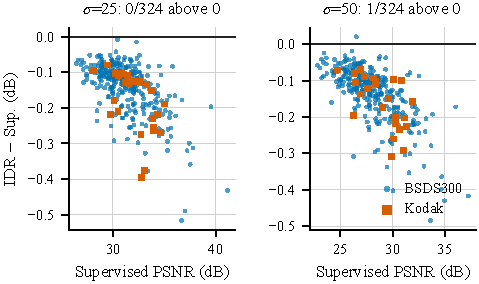
\includegraphics[width=\columnwidth]{fig_scatter.pdf}
\caption{Per-image PSNR, Fast IDR minus supervised (seed 0).}
\label{fig:scatter}
\end{figure}

\emph{Other noise} (Table~\ref{tab:img_other}).
\begin{itemize}
\item Binomial noise: IDR is within 0.4\,dB of the paper.
\item Impulse noise: IDR is $+1.04$\,dB (Kodak) and $-1.50$\,dB (BSDS300) from the paper. Our supervised impulse model is 1.60--3.61\,dB below the paper and below our own IDR, so we flag it as not reproduced.
\item Correlated noise: 7 of 8 cells are within $-0.16$ to $+1.42$\,dB. The exception, Kodak $g_1$ (30.01 vs.\ 37.46\,dB), comes from a model that matches the paper on BSDS300 $g_1$. The paper's own BM3D results are also inconsistent between datasets for this kernel, so we suspect the published entry.
\end{itemize}

\begin{table}[!t]
\centering
\caption{Non-Gaussian image noise, PSNR (dB), seed 0. (a) Binomial and impulse noise, $p=0.5$ (paper Table~5; the paper's text and table may swap the two row labels). (b) Spatially correlated noise, upstream kernels g1--g4 at upstream ``level 5'' (a variance of $5/255$); g5 is undefined in the released code. $\Delta$ = ours $-$ paper.}
\label{tab:img_other}
\resizebox{\columnwidth}{!}{%
\begin{tabular}{llcccccc}
\toprule
\multicolumn{8}{l}{(a) Binomial / impulse} \\
& & \multicolumn{3}{c}{Fast IDR} & \multicolumn{3}{c}{Supervised} \\
\cmidrule(lr){3-5}\cmidrule(lr){6-8}
Set & Noise & paper & ours & $\Delta$ & paper & ours & $\Delta$ \\
\midrule
Kodak & binomial & 31.63 & 31.78 & $+$0.15 & 31.84 & 32.41 & $+$0.57 \\
Kodak & impulse & 34.92 & 35.96 & $+$1.04 & 35.83 & 34.23 & $-$1.60 \\
BSDS300 & binomial & 32.18 & 31.81 & $-$0.37 & 32.32 & 31.51 & $-$0.81 \\
BSDS300 & impulse & 37.40 & 35.90 & $-$1.50 & 37.48 & 33.87 & $-$3.61 \\
\midrule
\multicolumn{8}{l}{(b) Spatially correlated} \\
Set & Kernel & BM3D (paper) & IDR (paper) & IDR (ours) & $\Delta$ & & \\
\midrule
Kodak & g1 & 31.56 & 37.46 & 30.01 & $-$7.45 \\
Kodak & g2 & 29.20 & 33.10 & 32.94 & $-$0.16 \\
Kodak & g3 & 31.38 & 41.88 & 42.27 & $+$0.39 \\
Kodak & g4 & 27.23 & 28.60 & 28.46 & $-$0.14 \\
BSDS300 & g1 & 26.77 & 29.83 & 29.73 & $-$0.10 \\
BSDS300 & g2 & 27.84 & 31.28 & 31.79 & $+$0.51 \\
BSDS300 & g3 & 29.59 & 38.22 & 39.64 & $+$1.42 \\
BSDS300 & g4 & 26.14 & 27.39 & 27.64 & $+$0.25 \\
\bottomrule
\end{tabular}}
\end{table}


\emph{Refinement} (Figs.~\ref{fig:refinement}--\ref{fig:convergence}). On Kodak $\sigma=25$, the Nr2N network scores 25.00\,dB applied directly to $x$ and 31.01\,dB with the Nr2N correction ($K=8$). Fast IDR scores 31.89\,dB. Most of the gain therefore comes from refinement, consistent with finding (ii) of~\cite{zhang2022idr}.

\begin{figure*}[!t]
\centering
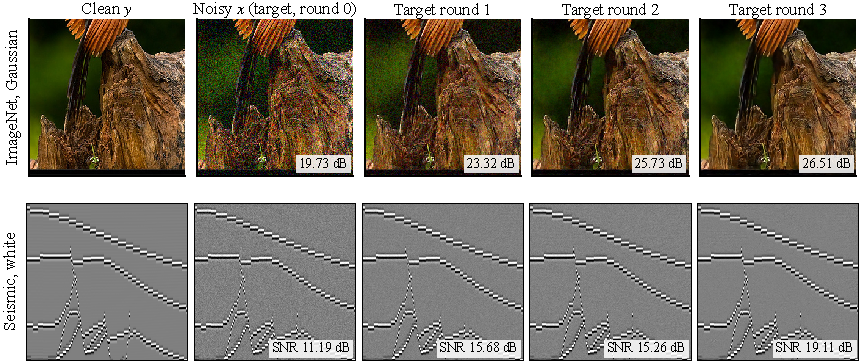
\includegraphics[width=\textwidth]{fig_refinement.pdf}
\caption{Fast IDR targets $x_i^{(m)}$ per round for one training crop. Top: image (PSNR). Bottom: seismic (SNR).}
\label{fig:refinement}
\end{figure*}

\begin{figure*}[!t]
\centering
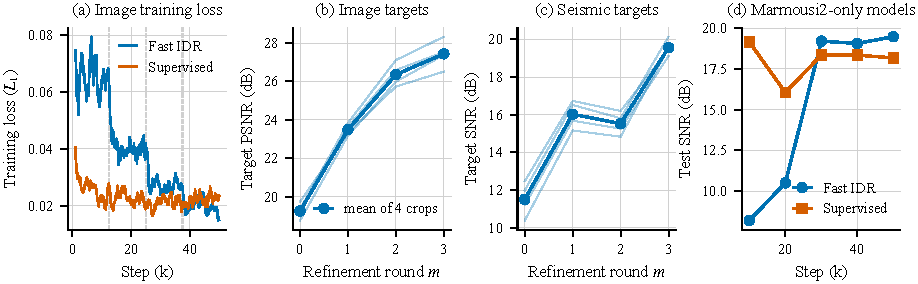
\includegraphics[width=\textwidth]{fig_convergence.pdf}
\caption{(a) Image training loss (dashed: teacher refreshes). (b), (c) Target quality per round. (d) Marmousi2-only models over training.}
\label{fig:convergence}
\end{figure*}

\subsection{Synthetic Seismic Data}
\emph{Data.} We use three synthetic datasets:
\begin{itemize}
\item \emph{Marmousi2}~\cite{martin2006marmousi2}: one $1001\times1400$ section of the NMO stack for training, and a disjoint 500-trace section for testing. The PreSTM, PostSTM and SRME versions of the test traces are used for testing only.
\item \emph{SEG/EAGE Overthrust and Salt}~\cite{aminzadeh1997}: converted to convolutional synthetics (Gardner density~\cite{gardner1974}, 30\,Hz Ricker wavelet, 4\,ms sampling), giving 280/9 and 235/10 train/test inlines.
\end{itemize}
Data rebuilt from public mirrors match our arrays to within $10^{-4}$ relative error. \emph{Joint} models train on all three surveys, \emph{per-survey} models on one.

\emph{Additive noise} (Table~\ref{tab:seis_add}, Figs.~\ref{fig:synth}--\ref{fig:fk}). Fast IDR comes within 1.2\,dB of supervised training on the training surveys. In 19 of 24 cells it is the best method that uses neither clean data nor a second noisy copy; in the other five, its fixed-noise variant leads by at most 0.25\,dB. Its margin is 0.19--4.66\,dB over oracle-$\sigma$ BM3D and 3.4--13.7\,dB over $f$-$x$ deconvolution. On the unseen Marmousi2 processing versions it beats supervised training in every case. Both networks preserve the signal cone in f--k. Above 75\,Hz, Fast IDR leaves more residual than supervised training but less than BM3D.

\begin{table*}[!t]
\centering
\caption{Synthetic seismic, additive noise: SNR (dB), joint models; sg IDR/Sup: mean of 3 seeds. $^\ast$Unseen processing. Bold/underline: best/second excluding N2N and supervised.}
\label{tab:seis_add}
\begin{tabular}{llccccccccc}
\toprule
Test & $\sigma$ & Input & Bandpass & $f$-$x$ & BM3D & Nr2N & IDR-fix & Fast IDR & N2N & Supervised \\
\midrule
\multicolumn{11}{l}{\emph{White Gaussian (sg)}} \\
Marmousi2 & 0.5 & 5.98 & 7.35 & 14.08 & \underline{19.12} & 18.65 & 16.76 & \textbf{19.47} & 19.86 & 19.46 \\
 & 1.0 & $-$0.04 & 2.79 & 9.04 & 14.68 & 15.57 & \underline{15.87} & \textbf{16.46} & 17.05 & 16.74 \\
M2 PreSTM$^\ast$ & 0.5 & 4.80 & 7.44 & 13.94 & 16.38 & \underline{16.40} & 15.15 & \textbf{17.37} & 16.40 & 15.67 \\
 & 1.0 & $-$1.22 & 2.01 & 8.63 & 12.28 & 13.36 & \underline{13.75} & \textbf{14.22} & 13.57 & 13.00 \\
M2 PostSTM$^\ast$ & 0.5 & 5.47 & 8.02 & 14.34 & \underline{16.34} & 16.16 & 15.35 & \textbf{17.08} & 16.01 & 15.30 \\
 & 1.0 & $-$0.55 & 2.66 & 9.14 & 12.29 & 13.25 & \underline{13.64} & \textbf{13.99} & 13.29 & 12.72 \\
M2 SRME$^\ast$ & 0.5 & 5.47 & 7.90 & 14.67 & 17.52 & \underline{18.00} & 16.14 & \textbf{18.52} & 18.07 & 17.62 \\
 & 1.0 & $-$0.56 & 2.62 & 9.50 & 13.95 & 15.35 & \underline{15.59} & \textbf{16.18} & 15.80 & 15.36 \\
Overthrust & 0.5 & 5.99 & 9.31 & 11.20 & 16.47 & 18.44 & \textbf{19.25} & \underline{19.07} & 19.88 & 19.96 \\
 & 1.0 & $-$0.03 & 3.39 & 7.51 & 12.07 & 14.26 & \textbf{15.45} & \underline{15.37} & 15.94 & 15.92 \\
Salt & 0.5 & 6.01 & 9.36 & 9.23 & 20.89 & 21.98 & \underline{22.99} & \textbf{23.24} & 24.00 & 24.42 \\
 & 1.0 & $-$0.01 & 3.42 & 6.80 & 16.06 & 17.90 & \underline{20.08} & \textbf{20.20} & 21.05 & 21.35 \\
\midrule
\multicolumn{11}{l}{\emph{Band-limited 5--60 Hz (sb)}} \\
Marmousi2 & 0.5 & 5.97 & 5.44 & 13.08 & \underline{17.88} & -- & 17.22 & \textbf{19.13} & -- & 18.78 \\
 & 1.0 & $-$0.04 & 0.31 & 7.92 & 13.82 & -- & \underline{15.61} & \textbf{15.96} & -- & 16.09 \\
M2 PreSTM$^\ast$ & 0.5 & 4.79 & 5.03 & 12.78 & \underline{15.21} & -- & 14.70 & \textbf{16.13} & -- & 14.43 \\
 & 1.0 & $-$1.23 & $-$0.65 & 7.49 & 10.91 & -- & \underline{12.74} & \textbf{13.13} & -- & 11.91 \\
M2 PostSTM$^\ast$ & 0.5 & 5.48 & 5.67 & 13.19 & \underline{15.23} & -- & 14.63 & \textbf{15.82} & -- & 14.37 \\
 & 1.0 & $-$0.56 & $-$0.00 & 8.04 & 11.00 & -- & \underline{12.59} & \textbf{12.99} & -- & 11.82 \\
M2 SRME$^\ast$ & 0.5 & 5.47 & 5.59 & 13.67 & \underline{16.54} & -- & 16.28 & \textbf{17.84} & -- & 16.99 \\
 & 1.0 & $-$0.55 & $-$0.01 & 8.45 & 12.85 & -- & \underline{15.02} & \textbf{15.48} & -- & 14.73 \\
Overthrust & 0.5 & 5.99 & 6.60 & 10.08 & 14.69 & -- & \textbf{17.51} & \underline{17.26} & -- & 18.06 \\
 & 1.0 & $-$0.03 & 0.64 & 6.28 & 9.72 & -- & \textbf{13.71} & \underline{13.62} & -- & 14.02 \\
Salt & 0.5 & 6.01 & 6.65 & 8.65 & 19.52 & -- & \textbf{22.33} & \underline{22.30} & -- & 23.51 \\
 & 1.0 & $-$0.01 & 0.67 & 5.80 & 14.04 & -- & \underline{18.67} & \textbf{18.70} & -- & 19.67 \\
\bottomrule
\end{tabular}
\end{table*}


\begin{figure*}[!t]
\centering
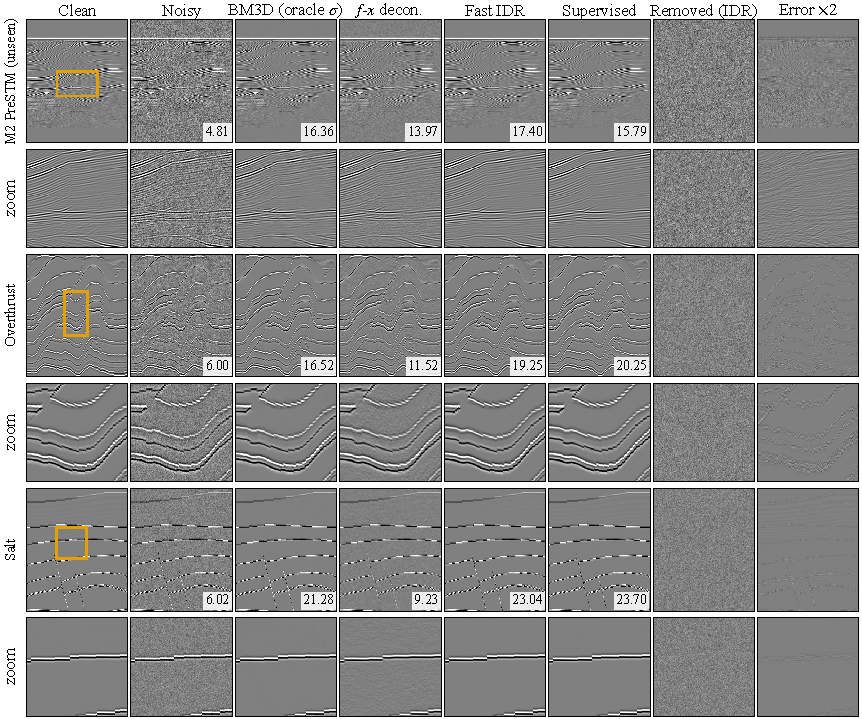
\includegraphics[width=\textwidth]{fig_synth.pdf}
\caption{White noise, $\sigma=0.5$, joint models. Labels: SNR (dB). Even rows: zoom on the orange box.}
\label{fig:synth}
\end{figure*}

\begin{figure*}[!t]
\centering
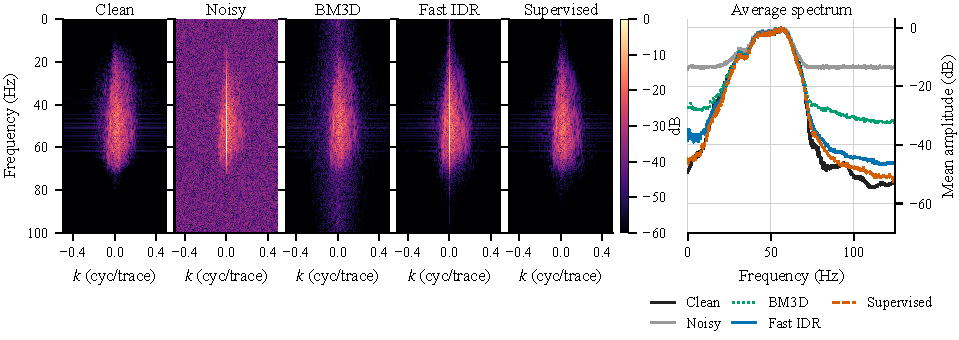
\includegraphics[width=\textwidth]{fig_fk.pdf}
\caption{Marmousi2 PreSTM (unseen), $\sigma=0.5$: f--k and average amplitude spectra.}
\label{fig:fk}
\end{figure*}

\emph{Sparse noise} (Table~\ref{tab:seis_sparse}). For spikes, supervised training leads by 3.2--5.1\,dB. For dead traces, it leads by up to 2.95\,dB (Marmousi2) and by at most 1.2\,dB elsewhere, and on Stratton trace interpolation beats both networks. As on images, refinement helps less when samples are destroyed rather than perturbed.

\begin{table}[!t]
\centering
\caption{Synthetic seismic, sparse noise: SNR (dB), joint models, seed 0. $^\ast$Unseen processing; $^\dagger$field data with added noise.}
\label{tab:seis_sparse}
\resizebox{\columnwidth}{!}{%
\begin{tabular}{llccccc}
\toprule
Test & Level & Input & Classical 1 & Classical 2 & Fast IDR & Sup. \\
\midrule
\multicolumn{7}{l}{\emph{Erratic spikes (ss), rate $p$}; classical: $f$-$x$, Median} \\
Marmousi2 & 0.05 & $-$1.51 & \underline{7.75} & $-$0.26 & \textbf{18.24} & 21.70 \\
 & 0.1 & $-$4.51 & \underline{5.00} & $-$0.26 & \textbf{15.39} & 18.61 \\
M2 PreSTM$^\ast$ & 0.05 & $-$2.69 & \underline{7.31} & $-$0.19 & \textbf{32.30} & 36.85 \\
 & 0.1 & $-$5.69 & \underline{4.52} & $-$0.22 & \textbf{28.25} & 32.55 \\
M2 PostSTM$^\ast$ & 0.05 & $-$2.00 & \underline{7.86} & $-$0.16 & \textbf{32.26} & 36.84 \\
 & 0.1 & $-$5.03 & \underline{5.09} & $-$0.21 & \textbf{28.67} & 32.67 \\
M2 SRME$^\ast$ & 0.05 & $-$2.01 & \underline{8.20} & $-$0.53 & \textbf{29.77} & 34.88 \\
 & 0.1 & $-$5.04 & \underline{5.36} & $-$0.54 & \textbf{26.19} & 31.16 \\
Overthrust & 0.05 & $-$1.50 & \underline{6.48} & 6.45 & \textbf{30.65} & 35.07 \\
 & 0.1 & $-$4.50 & 4.22 & \underline{6.05} & \textbf{26.85} & 31.13 \\
Salt & 0.05 & $-$1.47 & \underline{5.97} & 5.19 & \textbf{24.34} & 27.82 \\
 & 0.1 & $-$4.48 & 3.97 & \underline{4.94} & \textbf{21.51} & 25.87 \\
F3$^\dagger$ & 0.05 & $-$1.47 & 6.17 & \underline{9.36} & \textbf{21.16} & 20.36 \\
 & 0.1 & $-$4.50 & 3.94 & \underline{8.74} & \textbf{17.74} & 17.69 \\
Stratton$^\dagger$ & 0.05 & $-$1.90 & 6.69 & \underline{8.53} & \textbf{23.08} & 23.13 \\
 & 0.1 & $-$4.91 & 5.14 & \underline{8.07} & \textbf{19.20} & 19.81 \\
\midrule
\multicolumn{7}{l}{\emph{Dead traces (sd), fraction}; classical: Interp.} \\
Marmousi2 & 0.3 & 5.39 & -- & \underline{4.70} & \textbf{21.18} & 24.03 \\
 & 0.5 & 2.99 & -- & \underline{2.36} & \textbf{14.72} & 17.67 \\
M2 PreSTM$^\ast$ & 0.3 & 5.14 & -- & \underline{23.27} & \textbf{28.13} & 28.52 \\
 & 0.5 & 2.99 & -- & \underline{17.03} & \textbf{21.65} & 22.04 \\
M2 PostSTM$^\ast$ & 0.3 & 5.24 & -- & \underline{24.83} & \textbf{27.72} & 28.14 \\
 & 0.5 & 2.98 & -- & \underline{17.24} & \textbf{21.17} & 22.12 \\
M2 SRME$^\ast$ & 0.3 & 5.30 & -- & \underline{23.36} & \textbf{25.38} & 25.85 \\
 & 0.5 & 3.08 & -- & \underline{18.37} & \textbf{21.84} & 22.31 \\
Overthrust & 0.3 & 5.17 & -- & \underline{16.60} & \textbf{19.51} & 19.69 \\
 & 0.5 & 3.01 & -- & \underline{12.31} & \textbf{15.19} & 15.36 \\
Salt & 0.3 & 5.26 & -- & \underline{13.00} & \textbf{14.38} & 15.58 \\
 & 0.5 & 2.95 & -- & \underline{9.96} & \textbf{11.16} & 11.98 \\
F3$^\dagger$ & 0.3 & 5.27 & -- & \underline{17.67} & \textbf{18.07} & 17.75 \\
 & 0.5 & 3.01 & -- & \underline{12.44} & \textbf{12.77} & 12.69 \\
Stratton$^\dagger$ & 0.3 & 5.25 & -- & \textbf{13.87} & \underline{13.30} & 13.26 \\
 & 0.5 & 3.12 & -- & \textbf{10.58} & \underline{10.08} & 10.06 \\
\bottomrule
\end{tabular}}
\end{table}


\emph{Per-survey models} (Table~\ref{tab:perdataset}). For white noise, supervised training leads on Overthrust and Salt in every seed, by 0.51--1.35\,dB. On single-section Marmousi2, Fast IDR leads in every seed, by 0.61--1.30\,dB (and by 1.42\,dB for band-limited noise, seed 0), because supervised training overfits. In seed 0, supervised test SNR peaks at 10k steps (19.14\,dB) and ends at 18.17\,dB, while Fast IDR rises after the first refresh to 19.47\,dB (Fig.~\ref{fig:convergence}d). The fair reading is that Fast IDR matches early-stopped supervised training. Per-survey models fail on other surveys, often scoring below the input SNR, whereas the joint models do not. Within Marmousi2, the Marmousi2-only Fast IDR model transfers to the unseen processing versions better than the supervised model in every seed, but the margin depends strongly on the seed (1.66--4.20\,dB). For dead traces, supervised training leads by 0.41--1.27\,dB on Marmousi2 and 0.54--0.86\,dB on Salt, and the two tie on Overthrust. Both Marmousi2-only dead-trace models are 4.6--9.0\,dB above the joint models on Marmousi2, so for this noise type, training on the target survey matters more than the choice of method.

\begin{table*}[!t]
\centering
\caption{Per-survey vs.\ joint ($J$) models: own-survey SNR (dB; white noise: mean$\pm$sd over 3 seeds) and transfer (Fast IDR / supervised, mean over 3 seeds). $^\ast$Unseen processing.}
\label{tab:perdataset}
\begin{tabular}{lccccccccccc}
\toprule
& \multicolumn{4}{c}{White (sg)} & \multicolumn{2}{c}{Band-limited (sb)} & \multicolumn{2}{c}{Spikes (ss)} & \multicolumn{2}{c}{Dead traces (sd)} & sg \\
\cmidrule(lr){2-5}\cmidrule(lr){6-7}\cmidrule(lr){8-9}\cmidrule(lr){10-11}\cmidrule(lr){12-12}
Survey & IDR & Sup & IDR$_J$ & Sup$_J$ & IDR & Sup & IDR & Sup & IDR & Sup & fix \\
\midrule
Marmousi2 & 19.44$\pm$0.22 & 18.47$\pm$0.22 & 19.47 & 19.46 & 18.82 & 17.40 & 17.87 & 22.49 & 27.37 & 28.64 & 16.37 \\
Overthrust & 19.42$\pm$0.12 & 20.20$\pm$0.03 & 19.07 & 19.96 & 17.56 & 18.16 & 31.57 & 34.83 & 20.48 & 20.45 & 19.77 \\
Salt & 23.19$\pm$0.36 & 24.07$\pm$0.08 & 23.24 & 24.42 & 22.38 & 22.87 & 24.53 & 26.12 & 14.68 & 15.54 & 23.85 \\
\bottomrule
\end{tabular}

\vspace{4pt}
\begin{tabular}{lcccccc}
\toprule
Trained on $\downarrow$ / tested on $\rightarrow$ & Marmousi2 & M2 PreSTM$^\ast$ & M2 PostSTM$^\ast$ & M2 SRME$^\ast$ & Overthrust & Salt \\
\midrule
Marmousi2 & 19.44/18.47 & 15.72/12.65 & 15.27/12.31 & 17.69/15.21 & 3.31/3.32 & 4.90/4.63 \\
Overthrust & 3.04/4.01 & 10.15/9.28 & 10.26/9.47 & 10.89/8.90 & 19.42/20.20 & 17.52/18.13 \\
Salt & 5.30/5.72 & 9.16/7.00 & 9.30/7.12 & 9.80/7.54 & 14.06/12.54 & 23.19/24.07 \\
Joint & 19.47/19.46 & 17.37/15.67 & 17.08/15.30 & 18.52/17.62 & 19.07/19.96 & 23.24/24.42 \\
\bottomrule
\end{tabular}
\end{table*}


%=====================================================================
\section{Application to Real Field Data}\label{sec:field}
\emph{Data.} We use four public post-stack datasets, scaled to unit RMS:
\begin{itemize}
\item 2D land: NPR-A line 1~\cite{miller2000npra}, $\hat\sigma=0.383$;
\item 2D marine: NAMSS line WS82-611~\cite{namss}, $\hat\sigma=0.224$;
\item 3D land: Stratton~\cite{hardage1994stratton}, $\hat\sigma=0.092$;
\item 3D marine: F3~\cite{alaudah2019f3}, $\hat\sigma=0.054$.
\end{itemize}
Each 2D line provides two 512-trace test sections separated from the training traces by a 256-trace guard. \todo{Stratton/F3 train--test split and data source.}

\emph{Protocol.} Each model is assessed in two ways:
\begin{itemize}
\item \emph{Semi-synthetic test}: white noise is added and the original section serves as the reference, so only removal of the \emph{added} noise is measured.
\item \emph{Real-noise test}: models are applied to the raw sections and scored with the no-reference diagnostics.
\end{itemize}
Fast IDR is trained on each survey, either with one fixed realization of added noise (semi-synthetic test) or on the raw data with added noise $\sigma\sim U[0.5\hat\sigma,1.5\hat\sigma]$ (real-noise test). It is compared with the joint synthetic-corpus models.

\emph{Semi-synthetic results} (Table~\ref{tab:field_semi}, Fig.~\ref{fig:summary}b). Survey-trained Fast IDR is the best non-oracle method on all four datasets at $\sigma=0.5$, ahead of the best classical method by 2.13, 2.68, 1.17 and 1.13\,dB. On the 3D surveys it is within 0.13\,dB of, or above, a supervised oracle that treats the field section as clean. Synthetic-corpus models are 3.1--4.5\,dB worse on the 3D surveys, and on the 2D marine line they fall below the input SNR.

\begin{table*}[!t]
\centering
\caption{Field data with added white noise: SNR (dB). Best classical: $^B$BM3D, $^P$bandpass, $^F$$f$-$x$. Bold: best non-oracle. BM3D not run on 2D lines.}
\label{tab:field_semi}
\begin{tabular}{lcccccccc}
\toprule
& \multicolumn{2}{c}{2D land (NPR-A)} & \multicolumn{2}{c}{2D marine (NAMSS)} & \multicolumn{2}{c}{3D land (Stratton)} & \multicolumn{2}{c}{3D marine (F3)} \\
\cmidrule(lr){2-3}\cmidrule(lr){4-5}\cmidrule(lr){6-7}\cmidrule(lr){8-9}
Method & $\sigma$=0.5 & 1.0 & 0.5 & 1.0 & 0.5 & 1.0 & 0.5 & 1.0 \\
\midrule
Fast IDR, trained on the survey & \textbf{11.51} & \textbf{8.48} & \textbf{8.53} & \textbf{5.15} & \textbf{13.30} & \textbf{9.62} & \textbf{14.97} & \textbf{11.41} \\
\textit{Supervised on survey (oracle)} & -- & -- & -- & -- & 13.43 & 9.66 & 14.69 & 11.04 \\
Best classical & 9.38$^{P}$ & 5.92$^{F}$ & 5.85$^{P}$ & 2.76$^{F}$ & 12.13$^{B}$ & 8.42$^{B}$ & 13.84$^{B}$ & 10.04$^{B}$ \\
Fast IDR, synthetic corpus & 9.25 & 6.27 & 2.94 & 1.96 & 10.20 & 6.94 & 10.82 & 7.35 \\
Supervised, synthetic corpus & 9.63 & 6.25 & 3.31 & 2.09 & 10.25 & 6.87 & 10.48 & 7.28 \\
\textit{Input} & 6.01 & $-$0.02 & 4.93 & $-$1.09 & 5.58 & $-$0.44 & 6.01 & $-$0.01 \\
\bottomrule
\end{tabular}
\end{table*}


\emph{Real-noise results} (Table~\ref{tab:field_real}, Figs.~\ref{fig:field}--\ref{fig:field_spectra}). The survey-trained models behave differently on each dataset:
\begin{itemize}
\item \emph{2D land}: 0.15\% of the energy is removed, with leakage 0.118, and the removed component looks incoherent at $\times10$ gain. The synthetic-corpus models remove 6--10 times more energy, including reflectors ($|\rho|\approx0.37$).
\item \emph{2D marine}: 1.44\% is removed, mostly high-frequency and steeply dipping energy, but leakage is 0.320, so the separation is only partial. The synthetic-corpus models remove 34--64\% of the energy, including diffractions.
\item \emph{3D volumes}: 0.02--0.04\% is removed. Their residual noise is largely coherent (migration artefacts, acquisition footprint), which the additive noise model does not represent.
\end{itemize}
Two caveats apply to these diagnostics:
\begin{itemize}
\item Out-of-band fractions also count energy a model \emph{adds}. On the 2D land line above 75\,Hz, the spectrum of $r$ exceeds that of $x$ (Fig.~\ref{fig:field_spectra}).
\item The MAD estimate implies random noise of about 15\% (2D land) and 5\% (2D marine) of the energy, far more than is removed. $\hat\sigma$ is therefore best read as an upper bound.
\end{itemize}

\begin{table}[!t]
\centering
\caption{Real field noise: energy removed (\%), overall and in/out of 5--60\,Hz, and leakage.}
\label{tab:field_real}
\resizebox{\columnwidth}{!}{%
\begin{tabular}{llcccc}
\toprule
Data & Model & Removed & In band & Out of band & Leakage \\
\midrule
\multirow{4}{*}{\shortstack[l]{2D land\\$\hat\sigma$=0.383}} & Fast IDR, survey (raw + added noise) & 0.15 & 0.12 & 6.59 & 0.118 \\
 & Fast IDR, survey (fixed noisy copy) & 0.00 & 0.00 & 0.26 & 0.163 \\
 & Fast IDR, synthetic corpus & 1.44 & 1.30 & 28.60 & 0.373 \\
 & Supervised, synthetic corpus & 0.97 & 0.88 & 18.84 & 0.370 \\
\midrule
\multirow{4}{*}{\shortstack[l]{2D marine\\$\hat\sigma$=0.224}} & Fast IDR, survey (raw + added noise) & 1.44 & 0.46 & 4.74 & 0.320 \\
 & Fast IDR, survey (fixed noisy copy) & 0.04 & 0.01 & 0.13 & 0.300 \\
 & Fast IDR, synthetic corpus & 40.34 & 27.59 & 83.62 & 0.284 \\
 & Supervised, synthetic corpus & 33.97 & 20.53 & 79.46 & 0.290 \\
\midrule
\multirow{4}{*}{\shortstack[l]{3D land\\$\hat\sigma$=0.092}} & Fast IDR, survey (raw + added noise) & 0.04 & 0.01 & 0.18 & 0.054 \\
 & Fast IDR, survey (fixed noisy copy) & 0.03 & 0.01 & 0.09 & 0.511 \\
 & Fast IDR, synthetic corpus & 0.90 & 0.75 & 1.64 & 0.361 \\
 & Supervised, synthetic corpus & 0.73 & 0.79 & 0.57 & 0.338 \\
\midrule
\multirow{4}{*}{\shortstack[l]{3D marine\\$\hat\sigma$=0.054}} & Fast IDR, survey (raw + added noise) & 0.02 & 0.01 & 0.18 & 0.124 \\
 & Fast IDR, survey (fixed noisy copy) & 0.01 & 0.01 & 0.05 & 0.168 \\
 & Fast IDR, synthetic corpus & 1.09 & 0.75 & 4.64 & 0.311 \\
 & Supervised, synthetic corpus & 1.52 & 0.80 & 8.80 & 0.263 \\
\bottomrule
\end{tabular}}
\end{table}


\begin{figure*}[!t]
\centering
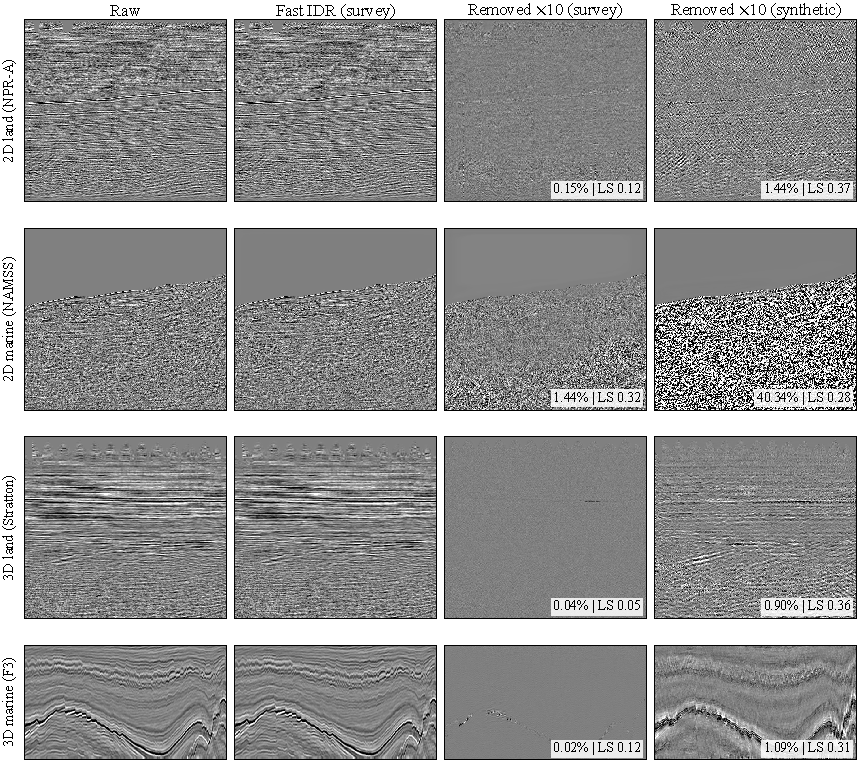
\includegraphics[width=\textwidth]{fig_field.pdf}
\caption{Real field noise: raw, survey-trained Fast IDR, and removed components ($\times10$). Labels: energy removed, leakage.}
\label{fig:field}
\end{figure*}

\begin{figure*}[!t]
\centering
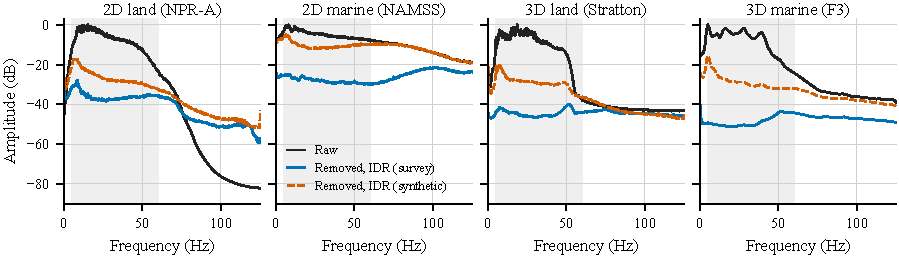
\includegraphics[width=\textwidth]{fig_field_spectra.pdf}
\caption{Amplitude spectra of raw data and removed components. Shaded: 5--60\,Hz.}
\label{fig:field_spectra}
\end{figure*}

%=====================================================================
\section{Results}\label{sec:results}
\emph{Seed variability} (Fig.~\ref{fig:summary}a). Across three seeds of the joint white-noise models:
\begin{itemize}
\item supervised training leads on Overthrust and Salt by 0.5--1.3\,dB;
\item Fast IDR leads on unseen processing by 0.84--2.16\,dB ($\sigma=0.5$) and 0.72--1.45\,dB ($\sigma=1.0$);
\item on the 3D field sections the two are within seed noise (sd up to 0.48\,dB).
\end{itemize}
For the per-survey white-noise models (three seeds), the sign of the Fast IDR versus supervised difference on each model's own survey is the same in every seed. Transfer scores vary much more between seeds (sd up to 2.06\,dB), so single-seed transfer numbers should not be trusted. Image training is far more repeatable, with seed sd $\le0.013$\,dB.

\begin{figure*}[!t]
\centering
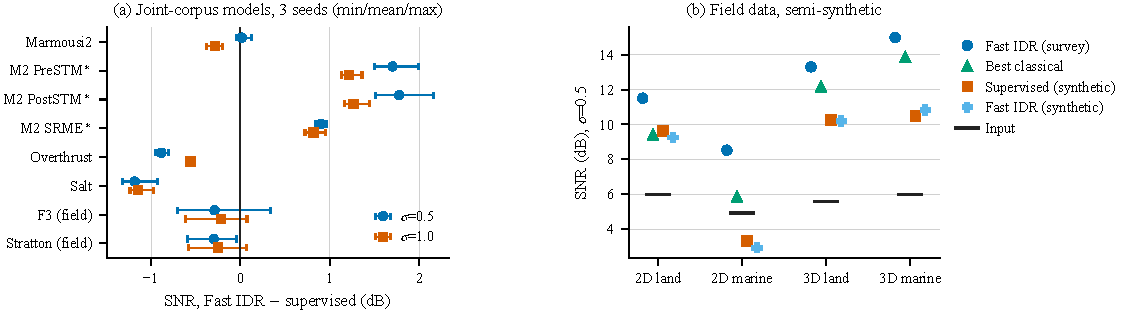
\includegraphics[width=\textwidth]{fig_summary.pdf}
\caption{(a) Fast IDR minus supervised SNR over three seeds; $^\ast$unseen. (b) Field data, $\sigma=0.5$; bar: input SNR.}
\label{fig:summary}
\end{figure*}

\emph{Ablations.}
\begin{itemize}
\item \emph{Refinement}: on Marmousi2, the Nr2N network scores 11.16\,dB applied directly and 18.65\,dB with the Nr2N correction ($K=8$), against 19.31\,dB for Fast IDR.
\item \emph{Fresh versus fixed noise}: replacing fresh noise draws with one fixed noisy copy costs 0.03--0.07\,dB on images. On single-section Marmousi2 it costs 1.91--3.10\,dB, but at most 0.46\,dB on Overthrust and Salt, so fresh noise matters when data are scarce.
\item \emph{Noise-model mismatch} (Table~\ref{tab:mismatch}): a white-noise model collapses on band-limited noise (3.07 vs.\ 16.09\,dB at $\sigma=1.0$), whereas a band-limited model handles white noise nearly as well (16.50 vs.\ 17.31\,dB).
\end{itemize}

\begin{table}[!t]
\centering
\caption{Noise-model mismatch: SNR (dB), mean over the synthetic test sets.}
\label{tab:mismatch}
\resizebox{\columnwidth}{!}{%
\begin{tabular}{lcccccc}
\toprule
& \multicolumn{3}{c}{Test: white (sg)} & \multicolumn{3}{c}{Test: band-limited (sb)} \\
\cmidrule(lr){2-4}\cmidrule(lr){5-7}
Trained on & 0.5 & 1.0 & 1.5 & 0.5 & 1.0 & 1.5 \\
\midrule
Fast IDR, sg & 20.51 & 17.31 & 14.99 & 13.24 & 3.07 & $-$1.40 \\
Supervised, sg & 21.15 & 17.90 & 15.47 & 14.41 & 2.76 & $-$1.86 \\
Fast IDR, sb & 19.87 & 16.50 & 13.88 & 19.56 & 16.09 & 13.51 \\
Supervised, sb & 19.84 & 16.44 & 12.55 & 20.12 & 16.59 & 13.69 \\
\bottomrule
\end{tabular}}
\end{table}


\emph{Reproduction fidelity} (Table~\ref{tab:drift}). Our earlier reproduction lost 1.37\,dB (IDR) and 0.98\,dB (supervised) on Kodak to a batch-192 epoch schedule, and a further 0.11/0.18\,dB to 128-pixel crops; protocol P removes both. None of the following explains the remaining gap: precision, the holdout split, test-noise or training seed, channel order, rounding, or the noise-sampling scheme. IDR stays about 0.45\,dB and supervised about 0.30\,dB below the paper, so most of the gap is common to both methods. The extra 0.15\,dB lost by IDR is unexplained; the untested 500k-step released schedule is the most plausible cause.

\begin{table}[!t]
\centering
\caption{PSNR change (dB) from each tested source of drift.}
\label{tab:drift}
\resizebox{\columnwidth}{!}{%
\begin{tabular}{lcc}
\toprule
Factor & IDR & Supervised \\
\midrule
\multicolumn{3}{l}{\emph{Training side}} \\
Batch 192, epoch schedule (earlier repro) & $-$1.37 & $-$0.98 \\
128-px crops (vs.\ 256-px, same split) & $-$0.11 & $-$0.18 \\
49k/1k train/holdout split & $-$0.03 & $+$0.01 \\
FP32 instead of TF32 (A1 control) & $-$0.04 & -- \\
Fixed noisy copy instead of fresh noise (A5) & $-$0.03 & -- \\
\midrule
\multicolumn{3}{l}{\emph{Inference side}} \\
BGR instead of RGB channel order & $-$0.05 & $-$0.02 \\
PSNR on float output (no uint8 rounding) & $+$0.01 & $+$0.01 \\
Clipping the noisy input to $[0,1]$ & $-$0.83 & $-$0.89 \\
BSDS300 test-100 split instead of all 300 ($\sigma$=25) & $-$0.36 & $-$0.38 \\
\bottomrule
\end{tabular}}
\end{table}


%=====================================================================
\section{Discussion}\label{sec:discussion}
IDR needs only noisy data and a noise model that can be sampled. It outperforms Nr2N trained under the same protocol wherever both were run, and it carries over to seismic data unchanged. Because its targets come from the data rather than from clean signals, it generalizes better than supervised training across processing versions and resists overfitting on a single section. Training on the target survey was the most useful configuration we tested.

Its main limitations are:
\begin{itemize}
\item \emph{Noise-model mismatch}: a white-noise model fails on band-limited noise, and the additive model misses the coherent noise of migrated volumes.
\item \emph{Sparse corruption}: spikes and dead traces leave a clear gap to supervised training.
\item \emph{Lack of theory}: there is no convergence guarantee for the refinement, and target quality did not increase monotonically in the seismic example (Fig.~\ref{fig:convergence}c).
\item \emph{Experimental coverage}: band-limited, spike and dead-trace runs use a single seed; we did not test input SNR below 0\,dB; the field references contain noise; and small edge artefacts appear, which we attribute to reflect padding.
\end{itemize}

In practice:
\begin{itemize}
\item train on the target survey;
\item prefer the band-limited noise model;
\item keep fresh noise draws on small surveys;
\item report leakage together with removed energy;
\item calibrate noise levels from noise-only windows rather than by MAD (untested).
\end{itemize}

%=====================================================================
\section{Conclusion}\label{sec:conclusion}
Under its stated protocol, Fast IDR reproduces in ranking and to within 0.30--0.54\,dB, but not at parity with supervised training (0.12--0.20\,dB below it in every row and seed). On seismic data it is a strong label-free denoiser for additive noise: it beats supervised training across processing versions and, trained on the target survey, beats every non-oracle method in semi-synthetic field tests. Low-leakage removal of real noise was observed only on the 2D land line. Next steps are noise models that represent coherent noise, and running the released 500k-step schedule.

\section*{Acknowledgment}
\todo{funding, compute, data providers (USGS, SEG, dGB/TU Delft, Bureau of Economic Geology); disclosure of AI assistance per venue policy.}

\bibliographystyle{IEEEtran}
\bibliography{references}
\end{document}
